% !TEX TS-program = pdflatex
% !TEX root = ../XJ_thesis.tex
%

\chapter{Introduction}
\label{sec:intro}

Nowadays, CCD or CMOS cameras are becoming more and more important in our daily life for their appplications in photography, security system, and robots, etc. The camera imaging pipeline is the key to transform the photons reflected by the real scene into the pixel values of an image, which can be displayed on a screen. During the camera imaging process, the noise is unavoidably generated due to many reasons. Two major reasons of noise generation are the discrete nature of light and the thermal agitation, which result in the photon shot noise and the dark-current noise, respectively. Image denoising aims to study how to recover the latent clean image from the captured noisy observation. 

This chapter will introduce how the noise is modeled in the imaging process, how the image denoising problem is formulated, how to evaluate the image denoising performance, and the major denoising methods. Finally, we will summarize the contributions and the structure of this thesis.

%\section{The Camera Imaging Pipeline}
%\label{sec:intro:general}

%The cameras capture the images and store as raw image formats. During the camera imaging pipeline, the photons are transformed into electronics by the photodiode in the camera sensor. The original sensor arrat (also called color filter array, or CFA) contains red, green, and blue channels, and these incomplete channels are transformed into the final RGB files via the raw converter. The camera imaging pipeline includes multiple stages such as reading raw image, black light subtraction, lens correction, demosaicing, noise reduction, white balancing, gamma curve, final color space conversion, etc \cite{browneccv2016}. Basically, a camera imaging pipeline includes demosaicing, white balancing and color space transform, gamut mapping, tone mapping, and JPEG compression \cite{crosschannel2016}. However, different cameras have varying structures and camera parameters, and hence resulting different imaging effects. Recently, there also exists learning based imaging pipelines which directly learn the  natural image priors from the RGB and raw images pairs.

\section{The Formulation of Image Denoising}
\label{sec:intro:current}

Due to the discrete nature of light and the thermal agitation, the camera sensors will have inaccurate measurements of image pixels. The measurement error is also called image noise. The noise generated during the imaging pipeline can be categorized into random noise, spatial non-uniformity noise, and quantization noise \cite{healey1994radiometric,Foipractical}. The random noise includes photon shot noise, dark current, and readout noise. The spatial non-uniformity noise includes fixed pattern noise (PRNU, DCNU) and CCD/CMOS specific noise. The quantization noise is the error generated in the final conversion from pixel measurements to pixel integers.

To better analyze the property of noise quantitatively, a simplified signal acquisition model \cite{Foipractical} (for each pixel) can be described as follows:
\begin{equation}
\label{e11}
\bm{P} = f((g_{cv}(\bm{C}+\bm{D})+\bm{N}_{reset})g_{out}+\bm{N}_{out})+\bm{Q},
\end{equation}
where $\bm{P}$ is the raw pixel value, and $f$ is the camera response function (usually $f$ is a linear function before attaining a saturation threshold). $\bm{C}$ is the number of absorbed electrons (charges) transformed from the photons via the photon-diodes in the camera sensor, which can be modeled by a Poisson distribution. $\bm{D}$ is the number of absorbed electrons generated in dark current by thermal generation, which is also often modeled by a Poisson distribution. $\bm{N}_{reset}$ is the thermal noise generated by the readout circuitry (or reset noise related to reset voltage), which can be well modeled by a Gaussian disribution. $\bm{N}_{out}$ is the readout noise, which is also modeled by a Gaussian distribution. $g_{cv}$ is the equivalent capacitance (EC) of the photo-diode and the gain factor during charge to voltage conversion. $g_{out}$ is the gain factor during voltage to pixel value conversion (readout). $\bm{Q}$ is the quantization error introduced during rounding to interger values, which is usually uniformly distributed and normally negligible compared to the readout noise。

After some merging and simplifying, the signal acquisition model (\ref{e11}) can be formulated as follows:
\begin{equation}
\label{e12}
\begin{split}
\textbf{P} 
&=f((g_{cv}(\textbf{C}+\textbf{D})+\textbf{N}_{reset})g_{out}+\textbf{N}_{out})+\textbf{Q},
\\
&=f(g_{cv}g_{out}(\textbf{C}+\textbf{D})+g_{out}\textbf{N}_{reset}+\textbf{N}_{out})+\textbf{Q},
\\
&=f(g\lambda+N_{R})+\textbf{Q},
\end{split}
\end{equation}
where $g = g_{cv}g_{out}$ is the overall camera gain factor, $\lambda=\textbf{C}+\textbf{D}$ is the number of electrons in pixel capacitor, and $N_{R}=g_{out}\textbf{N}_{reset}+\textbf{N}_{out}$ is the overall readout noise. In summary, the overall noise generated in the camera imaging pipeline can be modeled by a mixed Poisson and Gaussian distribution \cite{Foipractical}, which can also be approximated by a single Gaussian distribution according to the Central Limit Theorem.

To evaluate the performance of existing image denoising methods, the most common type of tested noise is the additive white Gaussian noise (AWGN) \cite{bm3d,ksvd}. The images with AWGN noise are corrupted by random values following Gaussian distribution with zero mean and a certain standard deviation (std). However, the real-world noise in the photographs captured by CCD or CMOS cameras is very complex and can hardly be modeled by a simple Gaussian distribution. The mixed Poisson and Gaussian distribution \cite{Foipractical} is also an ideal model for noise in the raw images captured by digital cameras. However, due the complex in-camera imaging pipeline, the noise in the output image will become much more complex than those in the raw image \cite{crosschannel2016,karaimer_brown_ECCV_2016}. This makes image denoising, especially real-world image denoising, a vary challenging task. The image denoising methods designed for the synthetic AWGN noise may fail when dealing with the real-world images captured by CCD or CMOS cameras.


As a classical yet fundamental problem for image quality enhancement in computer vision and photography, image denoising is generally modeled to recover the latent clean image $\bm{x}$ from the observed noisy image $\bm{y}=\bm{x}+\bm{n}$, where $\bm{n}$ is assumed to be the additive noise. In literature, most of the existing methods are designed for dealing with AWGN, where $\bm{n}$ follows Gaussian distribution $\mathcal{N}(0,\sigma^{2})$. The AWGN noise is a neat testing bed for evaluating the image denoising methods. However, for real-world noisy images, the image noise $\bm{n}$ is no longer Gaussian and signal independent, which makes the real-world image denoising problem much more difficult.


From the perspective of machine learning, image denoising can be viewed as a regression problem, in which a \textsl{plausible} clean image can be obtained from the infinite number of possible candidates. The word \textsl{plausible} means that the denoised image should look like the noisy image but without the noise corruption. As indicated in \cite{Bishop}, regression models, such as the famous least squares regression and LASSO \cite{lasso}, can be very inaccurate if we do not add proper prior to them. Similarly, image denoising problem would be very difficult if we do not employ suitable prior information of images. It is meaningful to exploit the prior information of the most \textsl{plausible} image given the input noisy image. The most commonly used framework in image denoising community is the Bayesian framework, which is also known as the maximum a-posterior (MAP) scheme. Under the MAP framework, the most \textsl{plausible} latent clean image is the one with maximum Bayesian probability for its noisy counterpart. The posterior probability can be computed with some explicit form which we will introduce in the following sections. In fact, the posterior probability can measure the distance of the latent clean image to the given noisy image. The closeness is usually measured by an $\ell_{2}$ norm of the difference between the two images. There are many candidate images which have the same $\ell_{2}$ norm distance to the given noisy image. But some images in the same distance are more \textsl{plausible} than the others due to the aspects of less artifacts, better structural preservation, and less remaining noise, etc. In general, more prior information of natural images can lead to better image denoising performance.


In order to evaluate the quality of denoised images, as well as compare the denoising performance of different methods, we need metrics of goodness for the denoised images. A natural problem is, how to measure the quality of the denoised image? To answer this question, we resort to the image quality assessment (IQA) metrics, which aim to provide solutions to measure the image quality for different applications such as image denoising, deblurring, super-resolution, etc. 

According to whether the reference clean image is available or not, existing IQA metrics can be roughly divided into two categories: 1) full reference IQA; and 2) no reference IQA. Full reference IQA metrics are based on the assumption that the clean image is available in order to compute a measure, while no reference IQA metrics can perform quality assessments without the reference image. The full reference IQA metrics include root-mean-square error (RMSE), peak signal-to-noise ratio (PSNR), and the structural similarity index (SSIM) \cite{ssim}, etc. Other IQA metrics include the multi-scale SSIM (MS-SSIM) \cite{msssim}, BLIINDS \cite{bliinds}, and BIQI \cite{biqi}, etc. A detailed survey of existing IQA algorithms is out of the scope of this thesis. Please refer to \cite{ssim} for more references.

\textbf{RMSE}: The root mean square error (RMSE) of the denoised image $\bm{y}\in\mathcal{R}^{M\times N}$ w.r.t. the original clean image $\bm{x}\in\mathcal{R}^{M\times N}$ is defined as the square root of the mean square error (MSE). The RMSE is usually employed to measure the $\ell_{2}$-norm distance between the denoised image and the original clean image. It is a full reference IQA metric which is closely related to the PSNR metric. Usually, smaller RSME value indicates better image quality. The definition of RMSE is:
\begin{equation}
\label{e13}
\text{RMSE}(\bm{x},\bm{y})
=
\sqrt{\frac{1}{MN}\sum_{i=1}^{M}\sum_{j=1}^{N}(\bm{x}_{ij}-\bm{y}_{ij})^{2}}.
\end{equation}



\textbf{PSNR}: peak signal-to-noise ratio (PSNR) is the most commonly used full reference IQA metric for many image restoration tasks including denoising. The definition of PSNR can be formulated as follows (for 8-bit image):
\begin{equation}
\label{e14}
\text{PSNR}
=
20\text{log}_{10}
(\frac{2^{8}}{\text{RMSE}(\bm{x},\bm{y})}).
\end{equation}
As we can see, PSNR is closely related to the $\ell_{2}$ norm distance between two images. The unit of PSNR is decibel (dB) and higher dB value indicates better image quality and lower RMSE. Though PSNR is very simple and intuitive, higher PSNR does not mean higher visual structural similarity. Hence, researchers resort to find alternative and better IQA metrics. 

\textbf{SSIM} \cite{ssim}: One seminal work in IQA is the structural similarity (SSIM) index metric, which is also a full reference IQA metric. In SSIM, each image patch is decomposed into three different components indicating three core informative parts of the original patch. The three components are luminance (mean value of the pixels in the patch), contrast (the standard deviation of the patch), and structure (the mean subtracted patch). SSIM takes into account the fact that the human visual system is very sensitive to the relative changes in luminance, rather than the absolute changes in luminance. The value range of SSIM is between 0 and 1, where higher value indicate higher similarity (SSIM=1 indicates that the two images are exactly the same), as well as better image quality. 

\textbf{Other IQA Metrics}: Besides the frequently used RMSE, PSNR and SSIM, there are many other IQA metrics for full reference and no reference IQA. For example, the MS-SSIM \cite{msssim} is a multi-scale extension of the original SSIM. Some examples in no reference IQA include BLIINDS \cite{bliinds} and BIQI \cite{biqi}. These IQA metrics capture the deviations from the expected statistics of the natural images. Specifically, BLIINDS measures the deviations from the expected histogram of certain features in DCT domain, while BIQI measures deviations from the expected distribution of wavelet coefficients in a multi-scale decomposition.

For different denoising tasks, we need different IQA metrics. For the synthetic noisy images corrupted by AWGN, we have the original clean images for the corresponding denoised images. Then we can directly measure the quality of the denoised image by some existing full reference IQA metrics. However, the original clean image does not always exists. For the real-world image denoising task, the corresponding clean image is hard to generate. A possible solution is to evaluate the image quality by human subjective or no reference IQA metrics. It should be noted that no IQA metric is perfect for the image denoising task, both in full reference and no reference cases. PSNR and SSIM are the de facto standard metrics in image restoration community. In addtion to the use of IQA metrics, it is essential to present the denoised images for human subjective evaluation.


\section{Existing Denoising Methods}

In this section, we will firstly review some well-known image denoising methods designed for AWGN, which is the most widely studied area in the literature. Though these methods are mainly proposed for the AWGN noise, the idea can be transfered into other image denoising tasks such as real-world image denoising. Then we will review some existing methods proposed for real-world noisy images.

\subsection{Synthetic Image Denoising}
\label{sec:review:sys}

Image denoising is a classical problem in low level vision. It has been extensively studied in the past decades, and is still an active research topic for that it provides an ideal test bed for image modeling techniques. In synthetic image denoising, the synthetic image noise is often assumed to be AWGN. Other types of synthetic image noise, e.g., Poisson noise and salt-and-pepper noise, are also widely studied in literature. The Poisson noise can be transformed into the additive noise after the generalized Anscombe transformation \cite{makitalo2013optimal}.

A number of image denoising methods for AWGN have been developed in past decades. Existing denoising methods can be categorized into three major categories: non-learning based methods, prior learning based methods, and discriminative learning based methods. 

% This category of methods include wavelet/curvelet transformation based methods \cite{softthresholding,bayesshrink,curvelet}, filtering based methods \cite{Tomasi1998,blsgsm,ple,nlm}, sparse and low-rank representation based methods \cite{bm3d,lssc,ncsr,nnm,wnnm},, and the other methods \cite{PeronaMalik1990,rudin1992nonlinear,osher2005iterative}.

\textbf{Non-learning based methods:} The filtering based methods, such as Gaussian filters, median filters, and bilateral filters \cite{Tomasi1998}, etc., design denoising filters to remove noise while preserving the details. The seminal work of bilateral filter \cite{Tomasi1998} is a non-linear, edge preserving, and smoothing filter for image denoising. It replaces the intensity of each pixel by a weighted average of intensity values from nearby pixels. The partial differential equation (PDE) based nonlinear anisotropic diffusion \cite{PeronaMalik1990} defines a class of efficient approaches, in which each diffusion step includes only the convolution operation with a few linear filters. The wavelet/curvelet transformation based methods perform image denoising in the transformed domain instead of the original image domain. By modeling the wavelet transform coefficients as Laplacian distributions, many wavelet shrinkage based denoising methods such as the classical soft-thresholding method \cite{softthresholding} have been proposed. Chang et al. modeled the wavelet transform coefficients as generalized Gaussian distribution, and proposed the BayesShrink \cite{bayesshrink} algorithm. Besides, curvelet based methods are also proposed for image denoising \cite{curvelet}. The TV based methods \cite{rudin1992nonlinear,osher2005iterative} have a principle that signals with excessive and possibly spurious detail have high TV, and hence reducing the TV of the signal tends to produce a close match to the original signal. It is widely accepted that natural image gradients exhibit heavy-tailed distributions \cite{weiss}, and the TV based methods \cite{rudin1992nonlinear,osher2005iterative} actually assume Laplacian distributions of image gradients for denoising. 

Most of previously mentioned methods exploit the local self-similarity prior of images, i.e., a pixel is similar to its neighboring pixels. The image NSS prior, which refers to the fact that the similar patches to a local patch can be far from it, has demonstrate much stronger image denoising performance. The nonlocal means (NLM) method \cite{nlm} has a basic idea that to build a pointwise estimate of the image where each pixel is a weighted average of pixels centered at regions that are similar to the region centered at the estimated pixel. The BM3D \cite{bm3d} method groups similar image patches into 3D data arrays, transform the image patches into the wavalet domain, then collaboratively filters the coefficients via shrinkage operations, and finally performs inverse transformation to recover the image. The BM3D algorithm has become a benchmark in image denoising. Mairal et al. \cite{lssc} proposed the LSSC algorithm to exploit NSS via group sparse coding. Dong et al. \cite{ncsr} unified NSS and local sparse coding into the so-called NCSR framework, which shows powerful image restoration capability. Since the NSS property has been demonstrated its effectiveness on image denoising task, low rank based methods \cite{nnm,wnnm} have also been proposed to exploit the intrinsic NSS property of nonlocal similar patches. For example, the work of WNNM \cite{wnnm} method achieves state-of-the-art performance for AWGN denoising. 

\textbf{Prior learning based methods:} The prior learning based methods learn the priors of natural images for image denoising. By considering the correlation of wavelet coefficients across scales, Portilla et al. \cite{blsgsm} proposed to use Gaussian Scale Mixtures for image modeling and achieved promising denoising performance. The Fields of Experts (FoE) \cite{foe} proposed by Roth and Black models the filtering responses with Student's t-distribution to learn filters through Markov Random Field (MRF) \cite{Bishop}. By viewing image patches as samples of a multivariate variable vector and considering that natural images are non-Gaussian, Zoran and Weiss \cite{epll,gmmnips} used Gaussian Mixture Model (GMM) to learn the distribution of natural image patches, and achieved state-of-the-art denoising perfromance. Yu et al. \cite{ple} used GMM to model image patches and perform denoising accordingly. 

The dictionary learning based methods remove the noise by thresholding the coefficients over the selected dictionary atoms. The seminal work of K-SVD \cite{ksvd,ksvdtsp} learns an overcomplete dictionary for the extracted image patches under the sparse representation framwork \cite{olshausen1997sparse,olshausen1996emergence}. The dictionary can be chosen from the off-the-shelf dictionaries (e.g., wavelets and curvelets), or it can be learned from natural image patches. The K-SVD method \cite{ksvd,ksvdtsp} has also been extended to color image denoising task \cite{srcolor,onlinedl}.

\textbf{Discriminative learning based methods:} The discriminative learning based denoising methods learn discriminative priors from pairs of clean and noisy images \cite{mlp,csf,tnrd, dncnn}. The multiple layer perception (MLP) \cite{mlp} has been introduced in the image denoising community and achieves good performance. Later, Schmidt and Roth proposed the cascade of shrinkage fields (CSF) to perform denoising efficiently \cite{csf}. Chen et al. proposed the trainable nonlinear reaction diffusion (TNRD) \cite{tnrd}, which achieves even better performance than CSF on image denoising as well as much faster speed. Recently, the residual network \cite{residualnetwork} has been applied into the image denoising task, and the developed DnCNN method \cite{dncnn} achieves state-of-the-art performance on image denoising.

\subsection{Real-world Image Denoising}
\label{sec:review:feature}

Most of the above mentioned methods focus on AWGN removal, however, the assumption of AWGN is too ideal to be true for real-world noisy images captured by CCD or CMOS cameras, where the noise is much more complex and varies with different scenes, cameras and camera settings (ISO, shutter speed, and aperture, etc.) \cite{crosschannel2016,karaimer_brown_ECCV_2016,dnd2017}. As a result, many denoising methods in literature, including those learning based methods, become less effective when applied to real-world noisy images.

During the last decade, several methods \cite{blsgsm,fullyblind,huber2011robust,rabie2005robust,cbm3d,Liu2008,noiseclinic,Zhu_2016_CVPR,
crosschannel2016,neatimage} have been proposed for real-world image denoising problem.\ Almost all of these methods follow a two-stage framework: first estimate the parameters of the noise model (usually assumed to be Gaussian or mixture of Gaussians (MoG)), and then perform denoising with the estimated noise model. To the best of our knowledge, the study of real-world image denoising can be traced back to the BLS-GSM method \cite{blsgsm}, where Portilla et al. proposed to use Gaussian scale mixture model in over-complete oriented pyramids to estimate the latent clean images. In \cite{fullyblind}, Portilla proposed to use a correlated Gaussian model for noise estimation of each wavelet subband. Based on the robust statistics theory \cite{huber2011robust}, Rabie modeled the noisy pixels as outliers, which could be removed via Lorentzian robust estimator \cite{rabie2005robust}. The CBM3D method \cite{cbm3d} is a representative color image denoising method and can be used in the real-world image denoising problem naturally. This method first transforms the RGB image into a luminance-chrominance space (e.g., YCbCr) and then applies the famous BM3D method \cite{bm3d} to each channel separately.

In \cite{Liu2008}, Liu et al. proposed the ``Noise Level Function'' to estimate the noise for each channel in natural images, and then use Gaussian conditional random field to obtain the latent clean image.\ Later, Lebrun el al. proposed a multiscale denoising algorithm called ``Noise Clinic'' \cite{noiseclinic} for blind image denoising task. This method generalizes the NL-Bayes \cite{nlbayes} to deal with signal and frequency dependent noise.\ Therefore, the methods \cite{noiseclinic,ncwebsite,Zhu_2016_CVPR} perform real-world color image denoising by concatenating the patches of RGB channels into a long vector.\ Zhu et al. \cite{Zhu_2016_CVPR} proposed a Bayesian method to approximate and remove the noise via a low-rank MoG model. The method in \cite{crosschannel2016} models the cross-channel noise in real-world noisy images as multivariate Gaussian and the noise is removed by the Bayesian non-local means filter \cite{kervrann2007bayesian}.\ The commercial software Neat Image \cite{neatimage} estimates the noise parameters from a flat region of the given noisy image and filters the noise accordingly. 


Despite the success of these methods, they also have clear limitations for the real-world image denoising task. On one hand, as suggested in \cite{Liu2008,noiseclinic}, Gaussian noise is assumed by \cite{fullyblind,rabie2005robust,Liu2008} and may be inflexible for the noise in real-world noisy images. Hence, better approximation to the real-world noise would bring better image denoising performance \cite{Liu2008,noiseclinic}. On the other hand, the real-world noise is signal dependent and have different statistics in different channels. It is hard to be modeled by explicit distributions such as Gaussian and MoG \cite{Liu2008,Leungtip,crosschannel2016,karaimer_brown_ECCV_2016,dnd2017}, and needs more complex modeling. Based on these observations, it is still needed to design robust and effective models for real-world image denoising.


\section{Contribution and Thesis Organization}
\label{sec:intro:new}

\begin{figure}[t!]
\centering
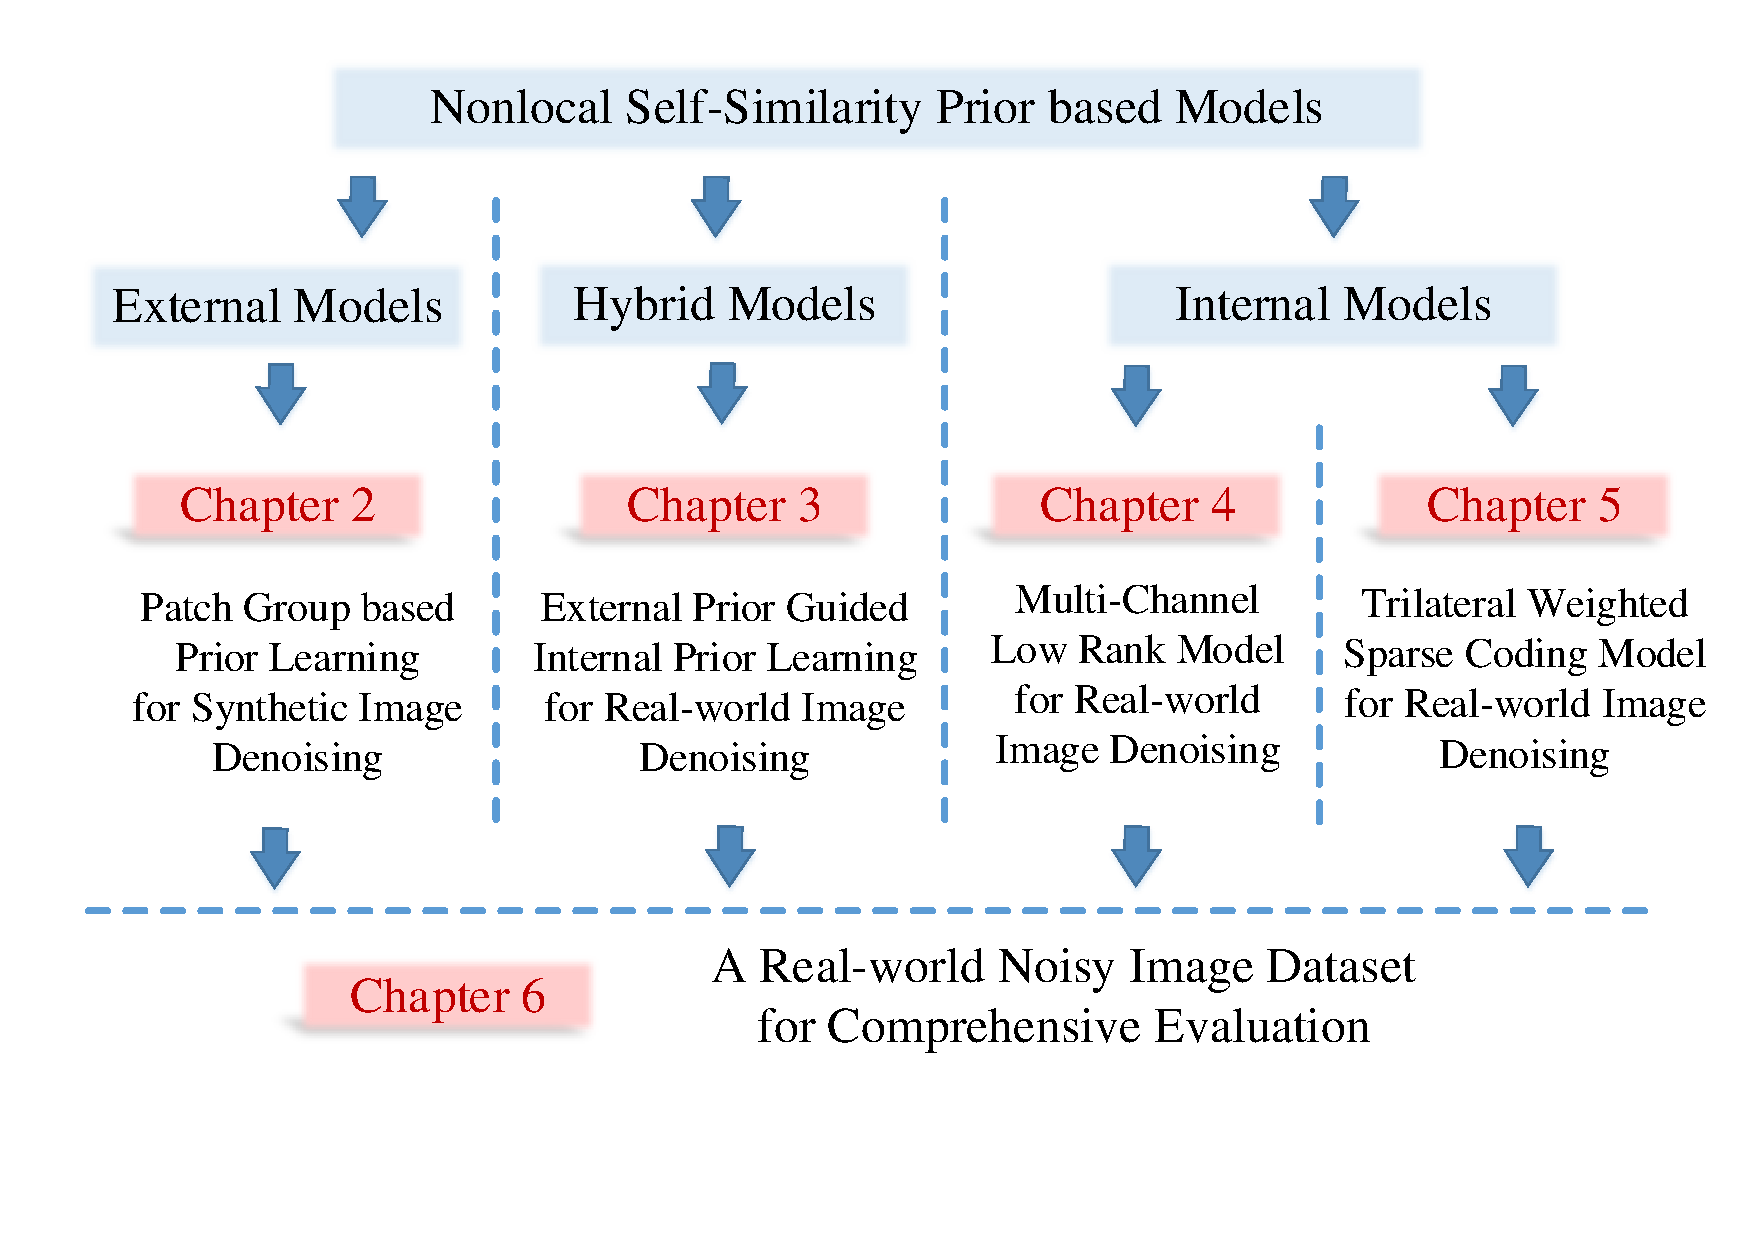
\includegraphics[width=1\linewidth]{images/ThesisOrganization.pdf}
\vspace{-20mm}
\caption{The organization of this thesis.}
\label{fig1-1}
\end{figure}

This thesis is mainly consisted of five works we have done during the PhD study, which focuses on designing new and better image denoising algorithms by proposing cutting-edge techniques for image modeling.\ The organization of the thesis is illustrated in Fig.\ \ref{fig1-1}.

\textbf{In the first work}, we propose to learn external nonlocal self-similarity (NSS) based priors and apply the learned model on removing AWGN noise. This is very different from the previous methods, which can be divided into three types: internal patch prior based methods \cite{ksvd,ple}, internal NSS prior based methods \cite{bm3d,lssc,ncsr,wnnm}, and external patch prior based methods \cite{epll}. As far as we know, this work is the first to learn the NSS priors of natural clean images, while previous works only utilize the NSS priors of input noisy image for online denoising. The advantages of this offline learning lie in that it can preserve the details of natural images while being much faster than most online denoising methods. The proposed method achieves state-of-the-art performance on AWGN removal effectively and efficiently. This work will be introduced in Chapter 2.

We then propose to exploit the NSS priors of natural images to deal with the complex noise in real-world noisy images. Specifically, we propose three methods for real-world image denoising, which are introduced as follows.

\textbf{In the second work}, we propose to learn the NSS prior from the external natural images, and then apply the learned external prior to guide the learning of the internal NSS prior of the input real-world noisy image. From the external perspective, the method can preserve the structures of natural images better than the internal methods, while from the internal perspective, the proposed method can recover the details of the input noisy image better than the external methods. The experiments on commonly used datasets demonstrate that the proposed method can achieve better performance than state-of-the-art real-world image denoising methods as well as a commercial software Neat Image \cite{neatimage}, which is embeded into the PhotoShop CS for image processing tasks. This work will be introduced in Chapter 3.


\textbf{In the third work}, we propose to employ the low rank model to describe the the internal NSS prior, basing on the fact that the similar image patches can be contanated as a matrix of low rank. We extend the WNNM model \cite{wnnm} to a multi-channel version to make it feasible for color image denoising. This method regards different channels in RGB images differently to adaptively process the real-world color noisy images. Experiments demonstrate that the proposed method can achieve better performance on real-world color image denoising than existing state-of-the-art methods, including some commercial software. This work will be introduced in Chapter 4.


\textbf{In the fourth work}, we propose to use the sparse coding based method with additional weighting scheme to deal with the real-world noisy images. We regard the noise in each local region as a Gaussian, and propose a triplely weighted scheme to deal with the complex real-world noise. Experiments show that the proposed method performs better and faster than the nuclear norm based method developed in Chapter 4. This work will be introduced in Chapter 5.


\textbf{In the final work}, to boost the research of real-world color image denoising, we construct a large benchmark dataset of real-world color noisy images. This dataset is collected by several representative cameras with comprehensive settings on contents, lighting, ISO, shutter, and aperture, etc. Based on this newly established dataset, we comprehensively evaluated existing denoising methods, including the methods designed for synthetic Gaussian noise and the methods designed especially for real-world noise. We believe that this new dataset will largely boost the research of the real-world image denoising. This work will be introduced in Chapter 6.


The structure of this thesis is organized as follows: in Chapter 2, we introduce the patch group based prior learning method for synthetic image denoising; in Chapter 3, we introduce the external prior guided internal prior learning method for real-world image denoising; in Chapter 4, we introduce the multi-channel weighted nuclear norm minimization based method for real-world image denoising; in Chapter 5, we introduce the trilateral weighted sparse coding based method for real-world image denoising; in Chapter 6, we introduce the real-world noisy image datasets, and comprehensively evaluate the proposed methods with the state-of-the-art denoising methods designed for synthetic AWGN noise and real-world noise, including a commercial software developed especially for real-world noise; in Chapter 7, we conclude this thesis and provide some future work directions.






